% !TEX root = ../main.tex

\chapter{Interpretation / Evaluation}
\label{ch:interpretation}

Evaluating creative software is not an easy task. Pease and Colton [27] divide it into two notions: \\
•	whether an idea or artefact is valuable or not, and\\
•	whether a system is acting creatively or not.\\
We would need to investigate each individual search result in terms of its value and creativity. This could be done by user ratings or satisfaction questionnaires. Rather than measuring the success of individual results we could look at evaluation them as one set instead, similar to the blind side-by-side comparisons by Bing or MillionShort .

The search results produced by our tool can be quite surprising sometimes and it not always clear how they connect to the initial query (especially if the inner workings of the algorithms are unknown), even if we identify through which function a result has been obtained. Obviously these keywords might not be helpful to users unfamiliar with the concept of pataphysics and might therefore appear rather nonsensical. Whilst there is a clear logic to each search result, they might appear anomalous to the user’s expectations if he received these results without knowing the philosophy of the search tool. The results could possibly appear random then, and would therefore likely to be detrimental to the user.

To prevent that, the level of interaction the user has with the system and the feedback the system gives to the user on decisions it is making will have a large influence on the overall effectiveness and appreciation of the tool. A quick and simple solution to this problem would be to add an icon to the side of each search result, which displays exactly how the original query was pataphysicalised.

\section{Evaluating Computer Creativity}

Creativity does not have a universally accepted definition. Creativity is a human quality and definitions don’t necessarily lend themselves to be applied to computers as well. There are aspects that come up in many, like novelty and value, but some that rarely pop up, like relevance and variety. Creativity can be studied at various \textbf{levels} (neurological, cognitive, and holistic/systemic), from different \textbf{perspectives} (subjective and objective) and \textbf{characteristics} (combinational, exploratory and transformative). Creativity should be seen as a continuum, there is no clear cut-off point or Boolean answer to say precisely when a person or piece of software has become creative or not.

Current evaluation methodologies have concentrated on only a handful of the points raised above, for example studying only the creative end-product itself (out of context), only judging it by its novelty objectively, assigning an arbitrary thresholds, etc. This also includes the assumption that machines "only" mimic humans and are therefore not judged by full potential.

\begin{comment}
  What does it mean, how can it be measured?

  Subjectivity vs objectivity is a theme throughout

  How is it defined and measured in humans, what can we just take directly from those concepts and apply them directly to machines and what needs to be completely redefined?
\end{comment}

This paper discusses issues related to the study of creativity in a computer science context. Two transdisciplinary fields of study have emerged from the variety of disciplines concerned. These are computational creativity and creative computing. The former lies at the cross section of artificial intelligence and cognitive science and the latter is mostly distinguished by its involvement in art. Creative computing focuses on the process of creativity rather than just the outcome as in computational creativity. In the remainder of this paper, CC will always denote creative computing unless otherwise specified.

\begin{comment}
  Many of these (if not all) spawn from the computational creativity discipline.

  Introduce the difference between human and computer evaluation/creativity?
\end{comment}

\begin{quote}
  "In research communities, approaches to the study of creativity differ in three main respects: 1) the type of research design, whether experimental, psychometric, observational etc. 2) the focus of the research, whether on human attributes cognitive processes or features of creative outcomes, and 3) the type of information that is used for the basis of evidence, by which is meant whether the time frame is present (real-time observation) or past (historical data) and whether the situation is artificial (laboratory) or natural (real world settings)." \citep[p.3]{Candy2012}
\end{quote}

\begin{comment}
  distinguishing between person’s and product’s creativity \citep[p.258]{Piffer2012}
  it is concluded that a person’s creativity can only be assessed indirectly (for example with self report questionnaires or official external recognition) but it cannot be measured \citep[p.258]{Piffer2012}
\end{comment}

\subsection{Output Minus Input}

It has been argued that "creativity may be seen as \textbf{output minus input}." \citep[p.2]{Pease2001}(my emphasis). The output in this case is the creative product but the input is not the process. Rather, it is the \textbf{inspiring set} (comprised of explicit knowledge such as a database of information and implicit knowledge input by a programmer) of a piece of software.

\begin{quote}
  "The degree of creativity in a program is partly determined by the number of novel items of value it produces. Therefore we are interested in the set of valuable items produced by the program which exclude those in the inspiring set." \citep[p.3]{Colton2001}
\end{quote}

\begin{quote}
  "We are interested in how a single agent can come up with something that is novel \textbf{relative to its initial state of knowledge}" \citep[p.72]{Ritchie2007}(his emphasis)
\end{quote}

"Output minus input" might easily be misinterpreted as "product minus process", however, that is not the case. In fact, Pease, Winterstein and Colton argue that "the process by which an item has been generated and evaluated is intuitively relevant to attributions of creativity" \citep[p.6]{Pease2001}, and that "two kinds of evaluation are relevant; the evaluation of the item, and evaluation of the processes used to generate it." \citep[p.7]{Pease2001}. If a machine simply copies an idea from its inspiring set then it just cannot be considered creative, and they need to be disqualified so to speak.

\begin{shaded}
  Summary\\
  •	output – input\\
  •	novelty + value\\
  •	product + process
\end{shaded}

\subsection{Measurable Attributes of Creativity}

Simon Colton came up with an evaluation framework called the \textbf{creative tripod}. The tripod consists of three behaviours a system or artefact should exhibit in order to be called creative. The three legs represent \textbf{skill, appreciation, and imagination} and three different entities can sit on it, namely the programmer, the computer and the consumer. Colton argues that the perception "that the software has been skillful, appreciative and imaginative, then, regardless of the behaviour of the consumer or programmer, the software should be considered creative. \citep[p.5]{Colton2008a} + \citep[p.5]{Colton2008b}. As such a product can be considered creative, if it appears to be creative. If not all three behaviours are exhibited, however, it should not be considered creative. \citep[p.5]{Colton2008a} + \citep[p.5]{Colton2008b}

\begin{quote}
  "Imagine an artist missing one of skill, appreciation or imagination. Without skill, they would never produce anything. Without appreciation, they would produce things which looked awful. Without imagination, everything they produced would look the same" \citep{Colton2008a}
\end{quote}

Pease, Winterstein and Colton suggest that all creative products must be \textbf{novel and valuable} \citep[p.1]{Pease2001} and provide several measures that take into consideration the context, complexity, archetype, surprise, perceived novelty, emotional response and aim of a product. In terms of the creative process itself they only discuss \textbf{randomness} as a measurable approach. Elsewhere, Pease et al discuss using \textbf{serendipity} as an approach \citep{Pease2013}.

Davide Piffer suggests that there are three dimensions of human creativity that can be measured, namely \textbf{novelty, usefulness/appropriateness and impact/influence}. \citep[p.258-259]{Piffer2012}. As an example of how this applies to measuring a person’s creativity he proposes citation counts \citep[p.261]{Piffer2012}. While this idea works well for measuring scientific creativity maybe, he does not explain how this would apply to a visual artist for example \footnote{http://www.artfacts.net seems to provide just that though.}.

Graeme Ritchie identifies three main criteria for creativity as \textbf{novelty, quality and typicality} \citep[p.72-73]{Ritchie2007}, although he argues that "novelty and typicality may well be related, since high novelty may raise questions about, or suggest a low value for, typicality" \citep[p.73]{Ritchie2007} \citep[see also]{Ritchie2001}. He proposes several evaluation criteria which fall under the following categories: \citep[p.91-92]{Ritchie2007} basic success, unrestrained quality, conventional skill, unconventional skill, avoiding replication and various combinations of those.

\begin{comment}
  This also somewhat suggests that variety is a criteria for creativity.
\end{comment}

Dan Ventura later suggested the addition of \textbf{variety and efficiency} to Ritchie’s model \citep[p.7]{Ventura2008}.

Geraint Wiggins introduced a formal notation and set of rules for the description, analysis and comparison of creative systems \citep{Wiggins2006} which is largely  based on Boden’s theory of creativity \citep{Boden2003}. The framework uses three criteria for measuring creativity: \textbf{relevance, acceptability and quality}.

Anna Jordanous proposed 14 key components of creativity, an ontology of creativity \citep[p.104-120]{Jordanous2012}, from a linguistic analysis of creativity literature which identified words that appeared significantly more often in discussions of creativity compared to unrelated topics. \citep[p.120]{Jordanous2012}.

\begin{quote}
  "The themes identified in this linguistic analysis have collectively provided a clearer ‘working’ understanding of creativity, in the form of components that collectively contribute to our understanding of what creativity is. Together these components act as building blocks for creativity, each contributing to the overall presence of creativity; individually they make creativity more tractable and easier to understand by breaking down this seemingly impenetrable concept into constituent parts."  \citep[p.120]{Jordanous2012}
\end{quote}

The 14 components Jordanous collated are: \citep[p.118-120]{Jordanous2012}
\begin{enumerate}
  \item Active Involvement and Persistence
  \item Generation of Results
  \item Dealing with Uncertainty
  \item Domain Competence
  \item General Intellect
  \item Independence and Freedom
  \item Intention and Emotional Involvement
  \item Originality
  \item Progression and Development
  \item Social Interaction and Communication
  \item Spontaneity / Subconscious Processing
  \item Thinking and Evaluation
  \item Value
  \item Variety, Divergence and Experimentation
\end{enumerate}

\begin{table}[htb]
  \begin{tabu}{XXXXXX}
  \toprule
  \textbf{Novelty}
  &
  \textbf{Value}
  &
  \textbf{Quality}
  &
  \textbf{Ephemeral Uncontrolled}
  &
  \textbf{Temporal Controlled}
  &
  \textbf{Purpose}
  \\ \midrule
  Originailty
  &
  Usefulness
  &
  Skill
  &
  Serendipity
  &
  Persistence
  &
  Intention
  \\ \midrule
  Newness
  &
  Appropriateness
  &
  Efficiency
  &
  Randomness
  &
  Results
  &
  Communication
  \\ \midrule
  Variety
  &
  Appreciation
  &
  Competence
  &
  Uncertainty
  &
  Development
  &
  Evaluation
  \\ \midrule
  Typicality
  &
  Relevance
  &
  Intellect
  &
  &
  Progression
  &
  Aim
  \\ \midrule
  Imagination
  &
  Impact
  &
  Acceptability
  &
  &
  Spontaneity
  &
  \\ \midrule
  &
  Influence
  &
  &
  Experimentation
  &
  &
  Independence
  \\
  \bottomrule
  \end{tabu}
\caption[Creativity attributes]{Summary of all creativity attributes}
\label{creatt}
\end{table}

\begin{comment}
  Temporal, spatial, ephemeral… what else?
\end{comment}

\begin{shaded}
  Summary\\
  •	Mimicking\\
  •	novelty + value + quality\\
  •	randomness + serendipity
\end{shaded}

\section{Problems with Evaluation}

Evaluating \textbf{human creativity} is problematic. Educational psychologist Richard Mayer identified several different approaches to human creativity research and each approach has its own methodologies and goals. \citep[p.453]{Mayer1999}

\begin{description}
  \item [Psychometric] (creativity as a mental trait): quantitative measurement, controlled environments, ability based analysis
  \item [Psychological] (creativity as cognitive processing): controlled environments, quantitative measurements, cognitive task analysis
  \item [Biographical] (creativity as a life story): authentic environments, qualitative descriptions, quantitative measurements
  \item [Biological] (creativity as a physiological trait): physiological measures
  \item [Computational] (creativity as a mental computation): formal modelling
  \item [Contextual] (creativity as a context-based activity): social, cultural and evolutionary context
\end{description}

There are many debates across the involved disciplines. Specifically, Mayer identified five big questions of human creativity research: \citep[p.450-451]{Mayer1999}

\begin{enumerate}
  \item Is creativity a property of people, products, or processes?
  \item Is creativity a personal or social phenomenon?
  \item Is creativity common or rare?
  \item Is creativity domain-general or domain-specific?
  \item Is creativity quantitative or qualitative?
\end{enumerate}

\begin{quote}
  "An important challenge for the next 50 years of creativity research is to develop a clearer definition of creativity and to use a combination of research methodologies that will move the field from speculation to specification." \citep[p.459]{Mayer1999}
\end{quote}

Taking these debates about human creativity and directly applying them to machines seems logical but may be the wrong and lazy approach. Adapting Mayer’s five big questions to machines does not seem to capture the real issues at play.

\begin{enumerate}
  \item Is creativity a property of programmers, users, machines, products, or processes?
  \item Is creativity a local, a network or an Internet phenomenon?
  \item Is creativity common or rare? (P or H creativity)
  \item Is creativity domain-general or domain-specific?
  \item Is creativity quantitative or qualitative?
\end{enumerate}

\begin{comment}
  \begin{itemize}
  \item Can a machine judge whether a human is creative?
  \item Is creativity a property of machines (hardware or software?)
  \item Is mimicking human creativity really enough and appropriate?
  \item Compare against "human creativity"? Or define machine creativity from scratch?
  \item Who is creative? The programmer or the program?
  \item Can creativity be objectively measured?
  \item Quantitative or qualitative?
  \item In respect to P or H creativity?
  \item Output minus input? (we don’t have the same strict judgement on humans)
  \item Is it the product or the process or both?
  \item Does context matter? (Blind deaf dumb person = computer?)
  \item Does time matter?
  \item Does purpose or intention matter?
  \item AGI vs AI? Artificial general creativity vs artificial creativity?
  \end{itemize}
\end{comment}

On a more practical level, there are various problems that arise when trying to evaluate computer creativity. Anna Jordanous found that "evaluation of computational creativity is not being performed in a systematic or standard way" \citep[p.2]{Jordanous2011}(her emphasis).

\section{Interpreting Computer Creativity}

\begin{comment}
(neurological, cognitive and systemic) in the computer sense!

Since most problems with evaluating creativity in computers (and humans alike) stems from the lack of a universal definition it seems logical to try and remedy this first and foremost.

Creativity is studied in many disciplines.
\begin{itemize}
  \item understanding the chemical mechanisms within the brain (neurological)
  \item understanding the thought processes associated with creativity (cognitive)
  \item understanding creativity in children and adults, novices and professionals
  \item understanding creativity in individuals and society (holistic)
\end{itemize}

Creativity is a continuum, which means that being creative and not being creative form the two distinct extreme ends of a scale.

\begin{quote}
  "a continuous sequence in which adjacent elements are not perceptibly different from each other, but the extremes are quite distinct" [OED]
\end{quote}

(subjective and objective)

How can we model Koestler’s bisociative creativity in computers?
Boden/Kaufman: Subjective and objective types (pandh or little-candbig-C) \citep{Boden2003, Kaufman2009} (product+process)

DIGITAL CREATIVITY ?!?!?! Mix between digital humanities and creative computing/computational creativity ---- see Digital Creativity Journal!!!!
Unified theory of creativity! (Koestler?)
Unified definition!

\begin{enumerate}
  \item What is the definition of creativity?
  \item Who is being creative? WHO
  \item What was the aim/intention, if any?
  \item What was the process, approach? HOW
  \item What factors influenced the person/process? WHERE
  \item What is the result/product, if any? Is it original, relevant? WHAT
  \item What is the impact, if any?
  \item What is the maintenance plan, if any?
\end{enumerate}
\end{comment}

\subsection{Linda Candy}

Evaluation is well established in HCI. HCI is not unsimilar to creativity. Design too.

I guess her work is meant mostly for "interactive art" while mine is meant for creative computing, but clearly there are many overlaps.

In HCI, historically, the focus has been on people as users deploying task oriented systems. The criteria for evaluation has largely been in terms of ease of use, task efficiency and effectiveness- usability. However, attributes such as speed and productivity are, for the most part, meaningless in the context of creative interactive experience. \citep[p.23]{Candy2012}

\begin{quote}
  Evaluation "is used to describe assessing and judging the value or worth of a particular idea or artifact both during the creative process and afterwards. Whether the process is systematic or ad hoc, evaluation depends upon criteria and measures that are situated and domain specific." \citep[p.7]{Candy2012}
\end{quote}

\begin{quote}
  "Whatever the context, evaluation is always tailored to the approach, needs, purpose and methodology of that context." \citep[p.7]{Candy2012}
\end{quote}

\begin{quote}
  "For evaluation to contribute to a successful outcome, the practitioner needs to have the necessary information including constraints on the options under consideration." \citep[p.7]{Candy2012}
\end{quote}

\begin{quote}
  "The matrix for evaluating creativity represents three standpoints: the capabilities of the creator, the audience, or more accurately, participant, experiences, and the features of the interactive systems as artworks. This initial matrix has been extended to include creative processes for both creator and audience participant (i.e. working practices and interaction experiences) and contextual factors in the form of the physical and technical environment in which the creative acts and events take place, including the influence of physical and technical resources and real world constraints." \citep[p.7-8]{Candy2012}
\end{quote}

\begin{quote}
  "Evaluation studies are well established in the field of Human-Computer Interaction (HCI) as well as interaction design contexts in general." \citep[p.8]{Candy2012}
\end{quote}

\begin{quote}
  "The evaluation of user, or rather, participant, experience of interactive artworks often involves measurement of aesthetic appreciation and the various engagement qualities which are dependent on personal traits, motivations, expectations, emotions and cognitive states of the audience. Those experiences that involve open-ended activity tend towards the creative end of human activity and, as such, are hardly ever measurable in quantitative ways."  \citep[p.8]{Candy2012}
\end{quote}

\begin{quote}
  "Evaluation is a key activity in creative design that can be revealed through documentation from design rationale. The introduction of rationale has been an important contribution to the quest for clarity and traceability in design decision-making. Design rationale may be thought of as structured records of design that support the understanding of decisions taken and allow designers to give better informed reconsideration to them at a later stage." \citep[p.9]{Candy2012}
\end{quote}

\begin{quote}
  "A software system can be viewed as an artifact that embodies implicit theoretical constructs that are realized as functional and operational requirements (Carroll and Campbell 1989). Structures are chosen because of their ability to achieve the intended functionality, and such choices may be evaluated against various criteria. During the design process, the ideas are modified and there is a clarification and refinement of intended functions and features. There may be additional factors arising from the context of the project that affect the way the design is carried out: for example the need to keep sight of general applicability whilst meeting the domain specific requirements, or the influence of the given hardware platform and software tools. Whatever the situation, the relationship between designers' decision making and the design outcome is not necessarily transparent and this is can be a problem when it comes to system maintenance. The explicit listing of decisions made during a design process, and the reasons why those decisions were made provides a means to record and communicate the reasoning and justification behind a design decision, including alternatives considered and constraints that affected the decision-making including why alternatives were rejected. The successful application of design rationale to software system design can provide a form of communication of intent from the designer to those who are to maintain the system." \citep[p.9]{Candy2012}
\end{quote}

\begin{quote}
  "A promising approach to the externalization of decision-making during the design process is being explored within practice-based research in the creative arts in the form of documented reflective practice. The approach builds upon a normal part of creative practice whereby practitioners draw and note ideas, designs and options in their sketch and notebooks. In this way, the documentation of tentative ideas and how they are worked into firmer proposals through testing and evaluation is a familiar and integral part of creativity. In practice-based research, documented reflective practice and empirical studies are frequently brought together." \citep[p.10]{Candy2012}
\end{quote}

\begin{quote}
  "The Multi-dimensional Model of Creativity and Evaluation (MMCE) shown in Figure 1 has four elements: people, process, product and context." \citep[p.11]{Candy2012}
\end{quote}

\begin{figure}[htb] % (here, top, bottom, page)
  \centering
  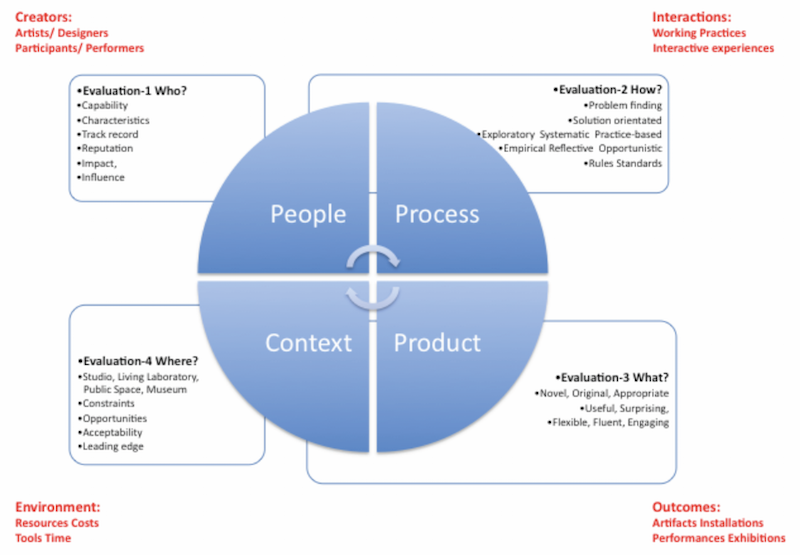
\includegraphics[width=\linewidth]{images/candy02.png}
\caption[Multi-dimensional Model of Creativity and Evaluation]{Candy's Multi-dimensional Model of Creativity and Evaluation}
\label{fig:candy02}
\end{figure}

\begin{figure}[htb] % (here, top, bottom, page)
  \centering
  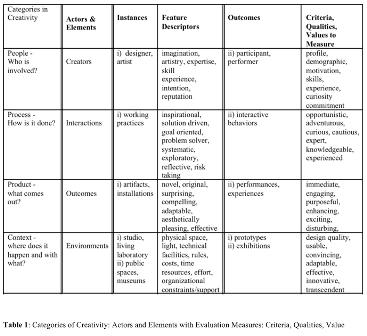
\includegraphics[width=\linewidth]{images/candy01.png}
\caption[Text for Table of Contents]{Caption text under figure}
\label{fig:candy01}
\end{figure}

\textbf{PEOPLE AS CREATORS}: \citep[p.14-15]{Candy2012}

Criteria for evaluating creator capability:
\begin{enumerate}
  \item The creator must be able to demonstrate an ability to create an artistic outcome where subject matter, ideas and technique are combined well to produce a coherent outcome.
  \item The creator must be able to demonstrate an ability to make work that is exploratory, creative and imaginative. Interesting ideas are presented in intelligent and surprising ways.
  \item In respect of Composition and Interpretation, the creator must be able to demonstrate the ability to:\\
  •	Select subject matter that is appropriate to a given theme\\
  •	Manipulate ideas and techniques in a coherent manner\\
  •	Express ideas visually (visual communication)\\
  •	Respond in an individual and personal way
\end{enumerate}

\textbf{PROCESS AS INTERACTION}: \citep[p.17]{Candy2012}

Criteria for evaluation can be expressed as follows
1. For a work to be deemed engaging, the participant should exhibit observable responses. There are likely to be different levels of engagement depending on whether or not the audience has had prior experience of this kind of artwork or installation or similar.\\
2. The participant responses demonstrate active engagement in three ways: Immediate, Sustained or Creative. The categories are defined as follows:\\
•	Immediate engagement: the work grabs immediate attention and yet is not so mundane as to create boredom.\\
•	Sustained engagement: the work must excite curiosity in the and also be accessible to a general audience.\\
•	Creative engagement: the work must excite immediate attention and encourage an audience to interact with it in a playful/purposeful way. As attention declines with familiarity and time, changes take place in the work that renew audience engagement.

\textbf{PRODUCT AS OUTCOME}: \citep[p.18]{Candy2012}

Typical features for judging artworks include composition, aesthetic, affect, content, and technique. Criteria for evaluation can be expressed as follows:

•	the composition of work should be coherent, exhibit shape and balance between order and complexity.\\
•	the work should exhibit outstanding visual and sound qualities in color, line and form.\\
•	the work should be pleasing, challenging, exciting, original etc.\\
•	the content should be appropriate and effective for the chosen subject matter\\
•	the execution should demonstrate high quality technique that fits the form.

It is interesting, therefore, to consider how criteria for judging the digital arts are specified by the Prix Ars Electronica, an international competition for Cyber Arts and the foremost event of its kind today.

Entries are judged by a Jury of experts in the order of their arrival and according to the following categories:

•	Aesthetics • Originality\\
•	Excellence of execution\\
•	Compelling conception\\
•	Innovation in technique of the presentation

\textbf{CONTEXT AS ENVIRONMENT}: \citep[p.21]{Candy2012}

Establishing a workable living laboratory for interactive art and evaluation involved setting down acceptance criteria for assessing whether or not a new interactive art system was ready to be deployed.

These included:
•	degree of robu\\stness of the art system in expectation of heavy public use
•	appropriate accessibility in respect of type of audience (e.g. children)\\
•	adherence to safety and house rules required by the museum\\
•	impact of other coinciding exhibits (sound, noise, light impacts)\\
•	attention to participant orientation and training\\
•	attention to art system maintenance by creator and technical support

\begin{quote}
  "we need to apply strategies for generating clear and unambiguous data that can be turned into meaningful information. From meaningful information, we can then derive understandings related to the context of use, the outcome of which might take the form of a coherent model." \citep[p.21]{Candy2012}
\end{quote}

\begin{quote}
  "Observation as a method for data collection raises issues as to its reliability in creativity evaluation. Data from observing creativity depends upon the interpretation of what the individual observer sees." \citep[p.22]{Candy2012}
\end{quote}

\begin{quote}
  "However, in order to ‘measure’ creativity, we have to conduct research outside of controlled laboratory conditions, and cannot rely on fixed criteria that can be applied to all cases. The shifting ground and the ever-changing contexts often renders consistency out of reach." \citep[p.22]{Candy2012}
\end{quote}

\begin{quote}
  "If the term 'measurement' does not match what we are doing within the creativity domain, then why do we still use this word?" \citep[p.22]{Candy2012}
\end{quote}

\begin{quote}
  "Whether an action is successful or unsuccessful depends on whether the intended result is achieved." \citep[p.23]{Candy2012}
\end{quote}

\begin{quote}
  "Measuring success is more likely to be dependent on factors such as whether or not the system has engaged the audience in a playful or immersive way or whether it has elicited curiosity or excitement or concentrated attention and so on." \citep[p.23]{Candy2012}
\end{quote}

\subsection{5 P’s: product, process, people, place and purpose}

\begin{quote}
  "One way of characterizing these processes is to use an alliteration that allows us to keep track of some of the core features of RRI in ICT, namely the four P's, which are: product, process, purpose and people. The purpose of using the four P's is to draw attention to the fact that, in addition to the widely recog- nized importance of both product and process of technical development, the purpose of the development needs to be considered and people involved in the innovation need to be incorporated in RRI." \citep[p.203]{Stahl2013} (my emphasis)
\end{quote}

\begin{comment}
  combine the 4 P’s with purpose//
  5 P’s: product, process, people, place and purpose//
  Why is the purpose important?//
  Interpreting or Measuring?//
  Maybe we should not be looking for metrics but rather guidelines for interpretations of creativity.
\end{comment}

\begin{draft}
  In the end I believe it is impossible to measure creativity objectively. I don’t just think it is impossible, I think it is unwise to try and do so. It would be silly to put a percentage on how creative something is just like it would be silly to say a certain product is 50percent ethical. In fact there are lots of parallels between (computer) ethics and (computer) creativity. Both are subjective, both are highly dependent on context.

  What is important is to study and consider the factors that influence our perception of whether something is creative (or ethical) and what the implications are.

  Creativity in a process or product will mean different things to different people, in different environments and contexts.
  Common sense.

  Just as there are people who just cannot see any creativity in in modern art, there will always be people who wont accept anything produced by a computer as creative.
\end{draft}


% -----------------------------

% \begin{comment}
% •	Brain operations per sec 1016 \citep[p.194]{Kurzweil2013}\\
% •	Japan’s K-computer has 1016 calculations per sec (10 petaflops)\\
% •	Blue brain project: 2023: 1017 bytes memory + 1018 flops \citep[p.125]{Kurzweil2013}
% \end{comment}
%
% Human Brain Project: \citep{Walker2012}
%
% Our brain consumes about 30W, the same as an electric light bulb, thousands of times less than a small supercomputer. \citep[p.17]{Walker2012}
%
% For environmental and business reasons, vendors have set themselves the goal of containing energy consumption to a maximum of 20 megawatts  \citep[p.41]{Walker2012}
%
% the 1 PFlop machine at the Jülich Supercomputing Centre could simulate up to 100 million neurons – roughly the number found in the mouse brain. \citep[p.41]{Walker2012}
%
% Cellular-level simulation of the 100 billion neurons of the human brain will require compute power at the exascale (1018 flops). \citep[p.41-42]{Walker2012}
%
% 2017 petascale 50petabytes memory + 50 petaflops + <=4MW power
%
% 2021 exascale 200petabyte memory + 1exaflop
%
% A second, equally important goal will be to prepare the procurement of the HBP Pre-exascale-supercomputer. By 2017/18, Jülich plans to procure a Big Data-centred system with at least 50 PBytes of hierarchical storage-class memory, a peak capability of at least 50 PFlop/s and a power consumption <= 4 MW. The memory and computational speed of the machine will be sufficient to simulate a realistic mouse brain and to develop first-draft models of the human brain. (The rest of the hardware roadmap targets an exascale machine in 2021/2022 with a capability of 1 EFlop/s and a hierarchical storage-class memory of 200 PB).\footnote{https://www.humanbrainproject.eu/high-performance-computing-platform}
%
% Chris Chatham: 10 Important Differences Between Brains and Computers \footnote{http://scienceblogs.com/developingintelligence/2007/03/27/why-the-brain-is-not-like-a-co/}
%
% \begin{enumerate}
% \item Brains are analogue; computers are digital
% \item The brain uses content-addressable memory
% \item The brain is a massively parallel machine computers are modular and serial
% \item Processing speed is not fixed in the brain; there is no system clock
% \item Short-term memory is not like RAM
% \item No hardware/software distinction can be made with respect to the brain or mind
% \item Synapses are far more complex than electrical logic gates
% \item Unlike computers, processing and memory are performed by the same components in the brain
% \item The brain is a self-organising system
% \item Brains have bodies
% \item	The brain is much, much bigger than any [current] computer
% \end{enumerate}
%
% Why Minds Are Not Like Computers \citep{Schulman2009}
% Software – Hardware == Mind – Brain ??? analogy
%
% "The power of the computer derives not from its ability to perform complex operations, but from its ability to perform many simple operations very quickly."
%
% Layers of abstraction in computers:\\
% 1.	user interface\\
% 2.	high level programming language\\
% 3.	machine language\\
% 4.	proessor microarchitecture\\
% 5.	Boolean logic gates\\
% 6.	transistors\\
%
% layers of abstraction in brain:\\
% 1.	personality?\\
% 2.	Thinking?\\
% 3.	Chemical /electrical signals/activity?\\
% 4.	Divided Brain regions/structure\\
% 5.	Neurons\\
% 6.	Dendrites (input) and axons (output)?\\
%
%
% Computers are faster and better than humans in many tasks already.
%
% \begin{quote}
% "The weaknesses of the computational approach include its assumption that cognition can be reduced to mathematics and the difficulty of including noncognitive factors in creativity." \citep[p.457]{Mayer1999}
% \end{quote}
%
% \subsection{Other}
%
% \begin{quote}
% "Currently many implementors of creative systems follow a creative-practitioner-type approach: produce a system then present it to others, whose critical reaction determines its worth as a creative entity. A creative practitioner’s primary aim, however, is to produce creative work, rather than to critically investigate creativity; in general this investigative aim is important in computational creativity research." \citep{Jordanous2011}
% \end{quote}
%
% purpose or intention shifts into focus here over production of products.
%
% \begin{quote}
% "Also, evaluation of novelty (or originality, newness) is often examined in the papers cited above according to how dissimilar the system’s artefacts are to previous output or other existing examples of creative output in that domain. On the other hand, appropriateness is often evaluated according to how similar the system’s output artefacts are to known examples. Hence across the field as a whole, there is a stark inconsistency as to whether to prioritise the generation of artefacts which are dissimilar from existing artefacts, or whether to pursue the generation of artefacts which are similar to existing artefacts, arising directly from the adoption of ‘novelty + value’ as the underlying model of creativity. Such a contradiction is clearly not helping the identification of coherent and consistent strategies to adopt across the field." \citep{Jordanous2012}
% \end{quote}
%
% \begin{quote}
% "In some cases, evaluative tests are conducted on the system which purportedly evaluate the system’s creativity but which actually only measure the system’s quality." \citep{Jordanous2012}
% \end{quote}
%
% But if quality is the "conformance to specifications" and the specification suggested creativity, then a good quality rating of a system would automatically mean it's creative, right?
%
% \begin{quote}
% "The key conclusion of the survey was that evaluation of computational creativity is not being performed in a scientifically rigorous manner:
% \begin{itemize}
% \item The creativity of a third of the 75 ‘creative’ systems was not critically discussed.
% \item Half the papers surveyed did not contain a section on evaluation.
% \item Only a third of systems presented as creative were actually evaluated on how creative they are.
% \item A third of papers did not clearly state or define criteria that their system should be evaluated by.
% \item Less than a quarter of systems applied existing creativity evaluation methodologies.
% \item Occurrences of evaluation by people outside the system implementation team were rare.
% \item Few systems were comparatively evaluated, to see if the presented system outperforms existing systems (a useful measurement of research progress).
% \item General principles of scientific method are not being followed by the community as a whole." \citep{Jordanous2012}
% \end{itemize}
% \end{quote}
%
% \begin{quote}
% "Reducing creativity to problem solving works when the creator is searching for an ideal solution which is not obvious, or if there is no single ideal solution but several candidates for a reasonable solution (Boden, 1994b)." \citep{Jordanous2012}
% \end{quote}
%
% \begin{quote}
% "One potential problem with Boden’s three views of creativity is that they all assume the existence of a conceptual space, or constrained set of possibilities, that the creative individual consciously reasons with in order to be creative." \citep{Jordanous2012}
% \end{quote}
